%==============================================================
%  EE201 -- Circuit Theory I
%  Lecture 7 : Circuit Graphs and the Incidence Matrix
%  M. Mert Ankaralı, METU EEE
%
%  Compile:  ./build.sh      (or: pdflatex EE201_Lecture_7.tex, twice)
%==============================================================
\documentclass[11pt,a4paper]{article}

%-------------------- packages --------------------------------
\usepackage[T1]{fontenc}
\usepackage[utf8]{inputenc}
\usepackage[english]{babel}
\usepackage{lmodern}
\usepackage[margin=2.3cm,top=2.0cm,bottom=1.9cm,headheight=14pt,headsep=9pt]{geometry}
\usepackage{amsmath,amssymb}
\usepackage{array,booktabs,tabularx}
\usepackage{enumitem}
\usepackage[table]{xcolor}
\usepackage{fancyhdr}
\usepackage{titlesec}
\usepackage{graphicx}
\usepackage[most]{tcolorbox}
\usepackage{tikz}
\usepackage[american,siunitx]{circuitikz}
\usetikzlibrary{matrix,arrows.meta,positioning,calc,decorations.pathmorphing,decorations.pathreplacing,decorations.markings,patterns,shapes.geometric}
\usepackage[colorlinks=true,allcolors=metured,breaklinks=true]{hyperref}

%-------------------- colour system ---------------------------
% One colour per physical quantity, used identically in the slides.
\definecolor{metured}{RGB}{155,27,48}    % headings, structure
\definecolor{metugray}{RGB}{88,89,91}
\definecolor{ccur}{RGB}{0,102,170}       % CURRENT  -- blue
\definecolor{cvolt}{RGB}{214,120,0}      % VOLTAGE  -- orange
\definecolor{cpow}{RGB}{23,128,74}       % POWER / ENERGY -- green
\definecolor{ccharge}{RGB}{124,60,160}   % CHARGE   -- purple
\definecolor{cflux}{RGB}{0,138,138}      % FLUX -- teal
\definecolor{boxgray}{RGB}{245,245,245}
\definecolor{copper}{RGB}{184,98,30}

\newcommand{\Icol}[1]{\textcolor{ccur}{#1}}
\newcommand{\Vcol}[1]{\textcolor{cvolt}{#1}}
\newcommand{\Pcol}[1]{\textcolor{cpow}{#1}}
\newcommand{\Qcol}[1]{\textcolor{ccharge}{#1}}
\newcommand{\Fcol}[1]{\textcolor{cflux}{#1}}

%-------------------- units (no siunitx dependency) -----------
\newcommand{\uni}[1]{\,\mathrm{#1}}
\newcommand{\A}{\uni{A}}   \newcommand{\V}{\uni{V}}
\newcommand{\W}{\uni{W}}   \newcommand{\J}{\uni{J}}
\newcommand{\Cb}{\uni{C}}  \newcommand{\s}{\uni{s}}
\newcommand{\Sie}{\uni{S}} \newcommand{\Wb}{\uni{Wb}}

%-------------------- layout ----------------------------------
\pagestyle{fancy}
\fancyhf{}
\lhead{\small\textcolor{metugray}{EE201 -- Circuit Theory I}}
\rhead{\small\textcolor{metugray}{Lecture 7: Circuit Graphs and the Incidence Matrix}}
\cfoot{\small\thepage}
\renewcommand{\headrulewidth}{0.4pt}

\titleformat{\section}{\large\bfseries\color{metured}}{\thesection.}{0.6em}{}
\titleformat{\subsection}{\normalsize\bfseries\color{metugray}}{\thesubsection.}{0.6em}{}
\titlespacing*{\section}{0pt}{1.4ex plus .3ex}{0.7ex}
\titlespacing*{\subsection}{0pt}{1.1ex plus .2ex}{0.5ex}

\setlist[itemize]{itemsep=2pt,topsep=3pt,parsep=0pt,leftmargin=1.5em}
\setlist[enumerate]{itemsep=2pt,topsep=3pt,parsep=0pt,leftmargin=1.7em}
\setlength{\parindent}{0pt}
\setlength{\parskip}{0.7ex plus .1ex}
\raggedbottom
\widowpenalty=10000
\clubpenalty=10000
\brokenpenalty=10000

%-------------------- boxes -----------------------------------
\newtcolorbox{definitionbox}[1]{enhanced,
  colback=metured!4, colframe=metured, boxrule=0.9pt,
  fonttitle=\bfseries, title={#1}, arc=2pt,
  left=7pt,right=7pt,top=5pt,bottom=5pt, before skip=7pt, after skip=7pt,
  before upper={\setlength{\parskip}{0.6ex plus .1ex}}}

\newtcolorbox{ideabox}[1][Key idea]{enhanced,
  colback=ccur!5, colframe=ccur, boxrule=0.9pt,
  fonttitle=\bfseries, title={#1}, arc=2pt,
  left=7pt,right=7pt,top=5pt,bottom=5pt, before skip=7pt, after skip=7pt,
  before upper={\setlength{\parskip}{0.6ex plus .1ex}}}

\newtcolorbox{examplebox}[1][Example]{enhanced,
  colback=cpow!4, colframe=cpow, boxrule=0.9pt,
  fonttitle=\bfseries, title={#1}, arc=2pt,
  left=7pt,right=7pt,top=5pt,bottom=5pt, before skip=7pt, after skip=7pt,
  before upper={\setlength{\parskip}{0.6ex plus .1ex}}}

\newtcolorbox{cautionbox}[1][Careful]{enhanced,
  colback=cvolt!6, colframe=cvolt, boxrule=0.9pt,
  fonttitle=\bfseries, title={#1}, arc=2pt,
  left=7pt,right=7pt,top=5pt,bottom=5pt, before skip=7pt, after skip=7pt,
  before upper={\setlength{\parskip}{0.6ex plus .1ex}}}

%-------------------- circuitikz defaults ---------------------
\ctikzset{bipoles/length=0.9cm, color=black,
          label/align=straight,
          bipoles/generic/height=0.28, bipoles/generic/width=0.62}
\tikzset{
  iar/.style={-{Stealth[length=2.2mm]}, ccur, thick},
  glab/.style={font=\footnotesize, text=metured},
  ttl/.style={font=\scriptsize\bfseries, text=metugray},
  capn/.style={font=\scriptsize, text=metugray, align=center},
  gnode/.style={circle, fill=metured, inner sep=0pt, minimum size=4.4pt},
  nlab/.style={circle, draw=metured, text=metured, font=\scriptsize, inner sep=0.7pt},
  blab/.style={font=\footnotesize, text=black!80},
  gbr/.style={black!75, thick, postaction={decorate, decoration={markings,
      mark=at position 0.56 with {\arrow{Stealth[length=2.5mm]}}}}},
  hal/.style={draw=cpow!60, line width=6pt, opacity=0.35, line cap=round, line join=round},
  elem/.style={draw=metugray, thick, fill=metulight},
}
\definecolor{metulight}{RGB}{243,240,241}
\newcommand{\ohm}{\,\Omega}

%  A circled node number, for the text and the matrices
\newcommand{\nd}[1]{\tikz[baseline=(c.base)]\node[nlab](c){#1};}
%  Branch current arrow beside the element from #1 to #2, on side #3 (90 = left, -90 = right),
%  with branch number #4
\newcommand{\brarr}[4]{%
  \draw[iar] ($(#1)!0.34!(#2)!0.34cm!#3:(#2)$) -- ($(#1)!0.66!(#2)!0.34cm!#3:(#2)$);
  \node[blab] at ($(#1)!0.5!(#2)!0.66cm!#3:(#2)$) {#4};}
%  A straight graph branch from #1 to #2, number #4 on side #3
\newcommand{\gbranch}[4]{%
  \draw[gbr] (#1) -- (#2);
  \node[blab] at ($(#1)!0.5!(#2)!0.28cm!#3:(#2)$) {#4};}
%  An incidence matrix with node labels on the left and branch numbers on top.
%  #1 name, #2 number of columns, #3 node labels, #4 rows (entries separated by \&)
\newcommand{\incmat}[4]{%
  \begin{tikzpicture}[baseline={([yshift=-0.6ex]#1.center)}]
    \matrix (#1) [matrix of math nodes, ampersand replacement=\&,
                  left delimiter={[}, right delimiter={]}, inner sep=1pt,
                  column sep=0.45em,
                  nodes={text width=1.35em, align=right, minimum height=1.25em,
                         inner sep=1pt}] {#4};
    \foreach \j in {1,...,#2}
      \node[font=\scriptsize, text=metugray, anchor=south east, inner sep=1pt]
        at ([yshift=2pt]#1-1-\j.north east) {\j};
    \foreach \lab [count=\i] in {#3}
      \node[nlab, left=11pt] at (#1.west |- #1-\i-1) {\lab};
  \end{tikzpicture}}
%  The four node positions of the bridge circuit N
\newcommand{\bridgecoords}{%
  \coordinate (n1) at (0,1.7);  \coordinate (n2) at (-1.5,0);
  \coordinate (n3) at (1.5,0);  \coordinate (n4) at (0,-1.7);}
\newcommand{\bridgenodes}{%
  \foreach \k/\pos in {1/above, 2/left, 3/right, 4/below}
    {\fill[metured] (n\k) circle (2.2pt); \node[nlab, \pos=3pt] at (n\k) {\k};}}

%==============================================================
\begin{document}

%-------------------- title block -----------------------------
\begin{center}
\begin{tcolorbox}[enhanced, colback=metured!5, colframe=metured, boxrule=1pt,
                  arc=3pt, left=10pt,right=10pt,top=7pt,bottom=7pt, width=\textwidth]
\begin{center}
  {\small\scshape Middle East Technical University}\\[2pt]
  {\small\scshape Department of Electrical and Electronics Engineering}\\[7pt]
  {\Large\bfseries\color{metured} EE201 -- Circuit Theory I}\\[4pt]
  {\large\bfseries Lecture 7: Circuit Graphs and the Incidence Matrix}\\[6pt]
  {\small M. Mert Ankaralı}
\end{center}
\end{tcolorbox}
\end{center}
\vspace{-0.5em}

\begin{center}
\small
\begin{tabular}{@{}l l@{}}
\toprule
\multicolumn{2}{@{}l}{\textbf{Colour code used in these notes and in the slides}}\\
\midrule
\Icol{$\blacksquare$}~current $i$ \quad \Vcol{$\blacksquare$}~voltage $v$ &
\textcolor{metured}{$\blacksquare$}~nodes \quad \textcolor{cpow}{$\blacksquare$}~a path in a graph\\
\bottomrule
\end{tabular}
\end{center}

%==============================================================
\section{Interconnection equations}

A circuit with $b$ branches has $2b$ unknowns: a voltage $\Vcol{v_k}$ and a current
$\Icol{i_k}$ for each branch $k$. The $2b$ equations that fix them come in two groups.

\begin{center}
\small
\begin{tabular}{@{}l c p{8.6cm}@{}}
\toprule
\textbf{Group} & \textbf{How many} & \textbf{What they describe}\\
\midrule
\textbf{element equations}        & $b$ & \emph{what} each element is: $\Vcol{v}=R\Icol{i}$,
                                          a source value, a dependent source, \dots\\
\textbf{interconnection equations} & $b$ & \emph{how} the elements are connected:
                                          $n-1$ KCL and $b-n+1$ KVL equations\\
\bottomrule
\end{tabular}
\end{center}

The interconnection equations do not depend on the elements at all. Replace a resistor by
a capacitor or by a source, keep the same wiring, and KCL and KVL do not change. So, to
write KCL and KVL, we may forget the elements and keep only the wiring. What is left is
the \textbf{graph} of the circuit.

This lecture builds the graph of a circuit and writes \emph{all} of its KCL equations as one
matrix equation. The same bookkeeping is how a circuit simulator stores a circuit: a list
of elements, each with the nodes it joins.

%==============================================================
\section{The graph of a circuit}

\begin{definitionbox}{Circuit graph}
The \textbf{graph} of a circuit is the circuit with every two-terminal element replaced
by a line segment, called a \textbf{branch}. The points where branches meet are the
\textbf{nodes}. Each branch gets a number and an arrow.

The graph records only \emph{which nodes each branch joins}, and in which direction it is
taken. Lengths, angles and the shape of the drawing carry no information.
\end{definitionbox}

\subsection{Procedure}
\begin{enumerate}
  \item Label each branch: $1, 2, \dots, b$.
  \item Assign a direction to each branch. The choice is \textbf{arbitrary}.
  \item Label each node: \nd1, \nd2, \dots, \nd{$n$}.
  \item Draw the graph: a dot for each node and an arrow for each branch.
\end{enumerate}

The arrow on branch $k$ is the \textbf{reference direction} of its current $\Icol{i_k}$.
As before we use associated reference directions, so the branch voltage $\Vcol{v_k}$ is
measured with $+$ at the tail of the arrow and $-$ at its head. Choosing an arrow does not
claim that the current really flows that way: if it flows the other way, $\Icol{i_k}$ comes
out negative.

\subsection{Example}

\begin{examplebox}[Example 7.1 --- the graph of a bridge circuit]
The circuit $\mathcal{N}$ below has six two-terminal elements, drawn as boxes because
their type does not matter here. Find its graph.

\begin{center}
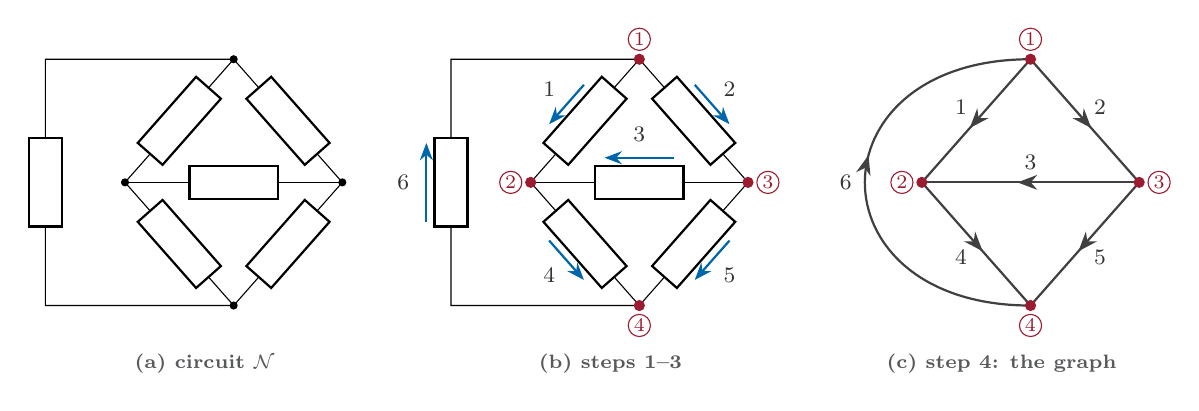
\begin{tikzpicture}[scale=0.92]
  \begin{scope}
    \bridgecoords
    \draw (n1) to[generic] (n2);  \draw (n1) to[generic] (n3);
    \draw (n3) to[generic] (n2);  \draw (n2) to[generic] (n4);
    \draw (n3) to[generic] (n4);
    \draw (n4) -- (-2.6,-1.7) to[generic] (-2.6,1.7) -- (n1);
    \foreach \k in {1,2,3,4} \fill (n\k) circle (1.6pt);
    \node[ttl] at (-0.4,-2.5) {(a) circuit $\mathcal{N}$};
  \end{scope}
  \begin{scope}[xshift=5.6cm]
    \bridgecoords
    \draw (n1) to[generic] (n2);  \draw (n1) to[generic] (n3);
    \draw (n3) to[generic] (n2);  \draw (n2) to[generic] (n4);
    \draw (n3) to[generic] (n4);
    \coordinate (s6) at (-2.6,-1.7); \coordinate (e6) at (-2.6,1.7);
    \draw (n4) -- (s6) to[generic] (e6) -- (n1);
    \brarr{n1}{n2}{-90}{1}  \brarr{n1}{n3}{90}{2}  \brarr{n3}{n2}{-90}{3}
    \brarr{n2}{n4}{-90}{4}  \brarr{n3}{n4}{90}{5}  \brarr{s6}{e6}{90}{6}
    \bridgenodes
    \node[ttl] at (-0.4,-2.5) {(b) steps 1--3};
  \end{scope}
  \begin{scope}[xshift=11.0cm]
    \bridgecoords
    \gbranch{n1}{n2}{-90}{1}  \gbranch{n1}{n3}{90}{2}  \gbranch{n3}{n2}{-90}{3}
    \gbranch{n2}{n4}{-90}{4}  \gbranch{n3}{n4}{90}{5}
    \draw[gbr] (n4) to[out=180, in=180, looseness=2.3] (n1);
    \node[blab] at (-2.55,0) {6};
    \bridgenodes
    \node[ttl] at (-0.4,-2.5) {(c) step 4: the graph};
  \end{scope}
\end{tikzpicture}
\end{center}

Steps 1--3 label the six branches, give each one an arrow (blue: the current reference),
and label the four nodes. Step 4 keeps only the dots and the arrows. The graph of
$\mathcal{N}$ has
\[
  \text{nodes } \{\nd1, \nd2, \nd3, \nd4\}, \quad n = 4;
  \qquad
  \text{branches } \{1, 2, 3, 4, 5, 6\}, \quad b = 6.
\]
Branch~6 is drawn curved only to keep it clear of the others; a straight arrow from \nd4 to
\nd1 would be the same graph.
\end{examplebox}

%==============================================================
\section{Elements with more than two terminals}

A two-terminal element becomes one branch. Some elements have more terminals: a
transistor has three, an integrated circuit can have many. Such an element cannot be one
line segment.

\begin{definitionbox}{A $k$-terminal element in the graph}
For an element with $k \ge 3$ terminals, choose one terminal as its \textbf{reference}
(the choice is arbitrary). Then draw $k-1$ branches, one from each of the other terminals
to the reference terminal.
\end{definitionbox}

Why $k-1$ branches, not $k$? A closed surface around the element is crossed by $k$
terminal currents, and KCL on that surface says they sum to zero. Only $k-1$ of them are
free; the last one follows. The voltages work the same way: the $k-1$ voltages measured
from the reference terminal fix every other voltage between terminals, by KVL. So $k-1$
branches, each with a current and a voltage, describe the element completely.

\begin{center}
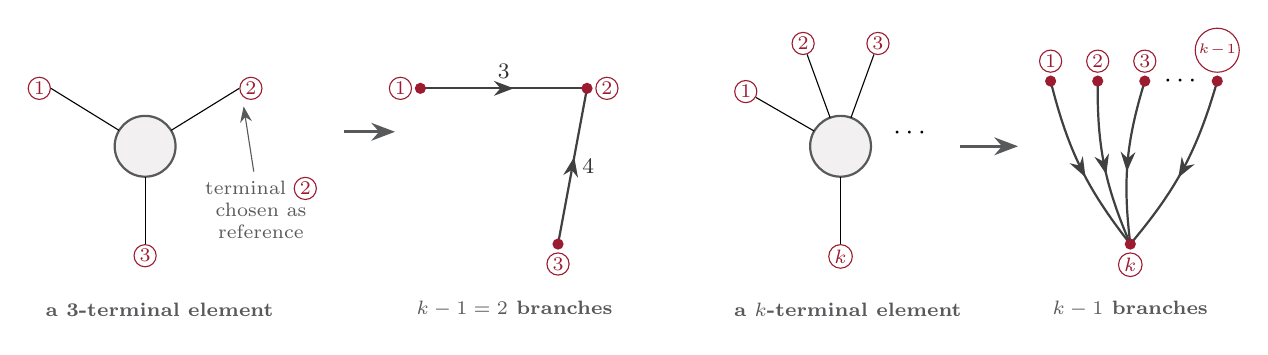
\begin{tikzpicture}[scale=0.92]
  % three-terminal element alone
  \begin{scope}
    \draw[elem] (0,0) circle (0.42);
    \draw (-0.36,0.22) -- (-1.3,0.8) node[nlab, left] {1};
    \draw (0.36,0.22) -- (1.3,0.8) node[nlab, right] {2};
    \draw (0,-0.42) -- (0,-1.35) node[nlab, below] {3};
    \node[capn] at (1.6,-0.85) {terminal \nd2\\ chosen as\\ reference};
    \draw[-{Stealth[length=2mm]}, metugray] (1.5,-0.35) -- (1.36,0.55);
    \node[ttl] at (0.2,-2.25) {a 3-terminal element};
  \end{scope}
  \draw[-{Stealth[length=3mm]}, very thick, metugray] (2.75,0.2) -- (3.45,0.2);
  \begin{scope}[xshift=5.1cm]
    \coordinate (t1) at (-1.3,0.8); \coordinate (t2) at (1.0,0.8); \coordinate (t3) at (0.6,-1.35);
    \draw[gbr] (t1) -- (t2);  \node[blab, above] at ($(t1)!0.5!(t2)$) {3};
    \draw[gbr] (t3) -- (t2);  \node[blab, right] at ($(t3)!0.5!(t2)$) {4};
    \foreach \k/\pos in {1/left, 2/right, 3/below}
      {\fill[metured] (t\k) circle (2.2pt); \node[nlab, \pos=3pt] at (t\k) {\k};}
    \node[ttl] at (0,-2.25) {$k - 1 = 2$ branches};
  \end{scope}
  % general k-terminal
  \begin{scope}[xshift=9.6cm]
    \draw[elem] (0,0) circle (0.42);
    \foreach \ang/\lab in {150/1, 110/2, 70/3}
      \draw (\ang:0.42) -- (\ang:1.35) node[nlab, anchor=\ang+180] {\lab};
    \draw (-90:0.42) -- (-90:1.35) node[nlab, below] {$k$};
    \node at (10:1.0) {$\cdots$};
    \node[ttl] at (0.1,-2.25) {a $k$-terminal element};
  \end{scope}
  \draw[-{Stealth[length=3mm]}, very thick, metugray] (11.25,0) -- (12.05,0);
  \begin{scope}[xshift=13.6cm]
    \coordinate (k) at (0,-1.35);
    \foreach \x/\lab in {-1.1/1, -0.45/2, 0.2/3}
      {\coordinate (u) at (\x,0.9);
       \draw[gbr] (u) to[bend right=12] (k);
       \fill[metured] (u) circle (2.2pt); \node[nlab, above=3pt] at (u) {\lab};}
    \coordinate (u) at (1.2,0.9);
    \draw[gbr] (u) to[bend left=12] (k);
    \fill[metured] (u) circle (2.2pt); \node[nlab, above=3pt, font=\tiny] at (u) {$k\!-\!1$};
    \node at (0.72,0.9) {$\cdots$};
    \fill[metured] (k) circle (2.2pt); \node[nlab, below=3pt] at (k) {$k$};
    \node[ttl] at (0,-2.25) {$k-1$ branches};
  \end{scope}
\end{tikzpicture}
\end{center}

A transistor is the most common case. With its emitter $E$ as the reference terminal it
becomes two branches: base to emitter, and collector to emitter.

\begin{center}
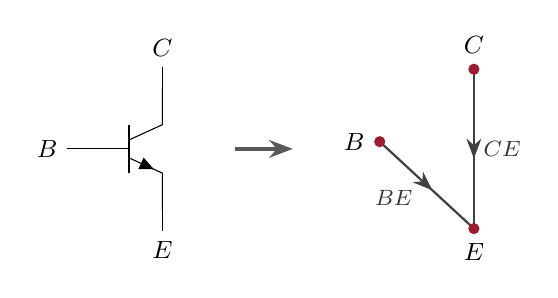
\begin{tikzpicture}[scale=0.92]
  \draw (0,0) node[npn](Q){};
  \draw (Q.B) -- ++(-0.4,0) node[left, font=\small] {$B$};
  \draw (Q.C) -- ++(0,0.3) node[above, font=\small] {$C$};
  \draw (Q.E) -- ++(0,-0.3) node[below, font=\small] {$E$};
  \draw[-{Stealth[length=3mm]}, very thick, metugray] (1.0,0) -- (1.8,0);
  \begin{scope}[xshift=3.0cm]
    \coordinate (B) at (0,0.1); \coordinate (C) at (1.3,1.1); \coordinate (E) at (1.3,-1.1);
    \draw[gbr] (B) -- (E); \draw[gbr] (C) -- (E);
    \node[blab, below left] at ($(B)!0.45!(E)$) {$BE$};
    \node[blab, right] at ($(C)!0.5!(E)$) {$CE$};
    \foreach \p/\pos in {B/left, C/above, E/below}
      {\fill[metured] (\p) circle (2.2pt); \node[font=\small, \pos=2pt] at (\p) {$\p$};}
  \end{scope}
\end{tikzpicture}
\end{center}

\begin{examplebox}[Example 7.2 --- a circuit with a 3-terminal element]
In the circuit below, element~1 joins nodes \nd1 and \nd2, element~2 joins \nd2 and \nd3,
and a 3-terminal element touches all three nodes. Find the graph.

\begin{center}
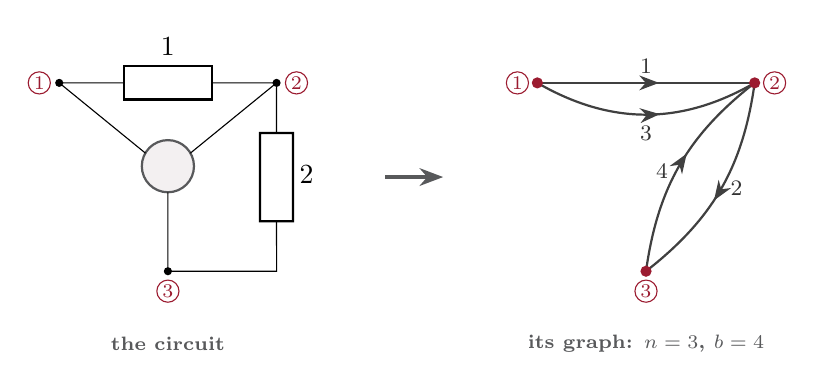
\begin{tikzpicture}[scale=0.92]
  \begin{scope}
    \coordinate (a) at (0,1.6); \coordinate (b) at (3,1.6); \coordinate (c) at (1.5,-1.0);
    \draw (a) to[generic, l=1] (b);
    \draw (b) to[generic, l=2] (3,-1.0) -- (c);
    \draw[elem] (1.5,0.45) circle (0.36);
    \draw (a) -- (1.19,0.63); \draw (b) -- (1.81,0.63); \draw (1.5,0.09) -- (c);
    \foreach \p/\k/\pos in {a/1/left, b/2/right, c/3/below}
      {\fill (\p) circle (1.6pt); \node[nlab, \pos=3pt] at (\p) {\k};}
    \node[ttl] at (1.5,-2.0) {the circuit};
  \end{scope}
  \draw[-{Stealth[length=3mm]}, very thick, metugray] (4.5,0.3) -- (5.3,0.3);
  \begin{scope}[xshift=6.6cm]
    \coordinate (a) at (0,1.6); \coordinate (b) at (3,1.6); \coordinate (c) at (1.5,-1.0);
    \draw[gbr] (a) -- (b);              \node[blab, above] at (1.5,1.6) {1};
    \draw[gbr] (a) to[bend right=30] (b); \node[blab] at (1.5,0.9) {3};
    \draw[gbr] (b) to[bend left=22] (c);  \node[blab] at (2.75,0.15) {2};
    \draw[gbr] (c) to[bend left=22] (b);  \node[blab] at (1.72,0.38) {4};
    \foreach \p/\k/\pos in {a/1/left, b/2/right, c/3/below}
      {\fill[metured] (\p) circle (2.2pt); \node[nlab, \pos=3pt] at (\p) {\k};}
    \node[ttl] at (1.5,-2.0) {its graph: $n = 3$, $b = 4$};
  \end{scope}
\end{tikzpicture}
\end{center}

Elements 1 and 2 give one branch each. For the 3-terminal element choose the terminal at
\nd2 as reference; it gives branch~3 (from \nd1 to \nd2) and branch~4 (from \nd3 to \nd2).
Branches 1 and 3 join the same two nodes; that is allowed, and so is the pair 2 and 4.
\end{examplebox}

A dependent source needs nothing new: it is already drawn as two branches, the branch that
senses the controlling variable and the branch of the source.

%==============================================================
\section{KCL on a circuit graph}

Every branch current flows along its own arrow. At each node, count a current
\textbf{leaving} the node with $+$ and a current \textbf{entering} it with $-$; KCL says
the sum is zero. For the graph of $\mathcal{N}$ in Example~7.1:

\begin{center}
\begin{minipage}[c]{0.36\linewidth}
\centering
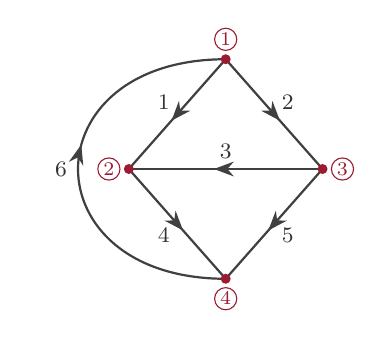
\begin{tikzpicture}[scale=0.82]
  \bridgecoords
  \gbranch{n1}{n2}{-90}{1}  \gbranch{n1}{n3}{90}{2}  \gbranch{n3}{n2}{-90}{3}
  \gbranch{n2}{n4}{-90}{4}  \gbranch{n3}{n4}{90}{5}
  \draw[gbr] (n4) to[out=180, in=180, looseness=2.3] (n1);
  \node[blab] at (-2.55,0) {6};
  \bridgenodes
\end{tikzpicture}
\end{minipage}%
\begin{minipage}[c]{0.6\linewidth}
\begin{alignat*}{7}
  &\nd1:\quad & \Icol{i_1} &{}+{}& \Icol{i_2} & & & & & & &{}-{}& \Icol{i_6} &= 0\\
  &\nd2:\quad & -\Icol{i_1} & & &{}-{}& \Icol{i_3} &{}+{}& \Icol{i_4} & & & & &= 0\\
  &\nd3:\quad & & &-\Icol{i_2} &{}+{}& \Icol{i_3} & & &{}+{}& \Icol{i_5} & & &= 0\\
  &\nd4:\quad & & & & & & &-\Icol{i_4} &{}-{}& \Icol{i_5} &{}+{}& \Icol{i_6} &= 0
\end{alignat*}
\end{minipage}
\end{center}

Nothing about the elements was used: the four equations come from the graph alone. Two
circuits with the same graph have the same KCL equations, whatever their elements are.

%==============================================================
\section{The incidence matrix}

The four equations above contain only the coefficients $+1$, $-1$ and $0$. Collect them
in a matrix, and collect the currents in a vector:
\[
  \incmat{Aa}{6}{1,2,3,4}{%
     1 \&  1 \&  0 \&  0 \&  0 \& -1\\
    -1 \&  0 \& -1 \&  1 \&  0 \&  0\\
     0 \& -1 \&  1 \&  0 \&  1 \&  0\\
     0 \&  0 \&  0 \& -1 \& -1 \&  1\\}
  \;
  \begin{bmatrix}
    \Icol{i_1}\\ \Icol{i_2}\\ \Icol{i_3}\\ \Icol{i_4}\\ \Icol{i_5}\\ \Icol{i_6}
  \end{bmatrix}
  =
  \begin{bmatrix} 0\\ 0\\ 0\\ 0 \end{bmatrix}
  \qquad\Longleftrightarrow\qquad
  A_a\,\Icol{\mathbf{i}} = \mathbf{0} .
\]
Rows are labelled by nodes, columns by branches. A matrix that stores the graph like this
is a \textbf{circuit matrix}. There are several; the first and most basic is this one.

\begin{definitionbox}{Incidence matrix}
For a graph with $n$ nodes and $b$ branches, the \textbf{incidence matrix} $A_a$ is the
$n \times b$ matrix with entries
\[
  a_{ij} =
  \begin{cases}
    +1 & \text{if branch } j \text{ leaves node } i,\\
    -1 & \text{if branch } j \text{ enters node } i,\\
    \phantom{+}0 & \text{otherwise.}
  \end{cases}
\]
With the \textbf{branch current vector}
$\Icol{\mathbf{i}} = [\,\Icol{i_1}\ \Icol{i_2}\ \cdots\ \Icol{i_b}\,]^{T}$, KCL at every node
of the circuit is the single equation $A_a\,\Icol{\mathbf{i}} = \mathbf{0}$.
\end{definitionbox}

The subscript $a$ stands for \emph{all}: every node has a row. The matrix can be read in
two directions.

\begin{itemize}
  \item \textbf{A row} is a node. Its nonzero entries are the branches that touch that
        node, and the row times $\Icol{\mathbf{i}}$ is the KCL equation at that node.
  \item \textbf{A column} is a branch. It has exactly one $+1$ (the node the branch
        leaves) and exactly one $-1$ (the node it enters). Column~3 above has $+1$ in row
        \nd3 and $-1$ in row \nd2: branch~3 goes from \nd3 to \nd2.
\end{itemize}

The columns hold all of the graph: from $A_a$ alone one can redraw the graph, arrows
included. Reversing the arrow of a branch flips the sign of its column, and nothing else.

%==============================================================
\section{Review: linear dependence}

\begin{definitionbox}{Linear dependence}
Let $\mathbf{v}_1, \mathbf{v}_2, \dots, \mathbf{v}_k$ be vectors of the same size. If there
are real numbers $\alpha_1, \alpha_2, \dots, \alpha_k$, \textbf{not all zero}, with
\[
  \alpha_1\mathbf{v}_1 + \alpha_2\mathbf{v}_2 + \dots + \alpha_k\mathbf{v}_k = \mathbf{0},
\]
the vectors are \textbf{linearly dependent}. Otherwise --- if the only such numbers are
$\alpha_1 = \dots = \alpha_k = 0$ --- they are \textbf{linearly independent}.
\end{definitionbox}

If the vectors are dependent, at least one of them is a combination of the others: pick
an $\alpha_m \neq 0$ and solve for $\mathbf{v}_m$.

\begin{examplebox}[Example 7.3 --- dependent or not?]
\[
  \begin{bmatrix} 1\\ 0 \end{bmatrix},\ \begin{bmatrix} 0\\ -1 \end{bmatrix}
  \ \text{are independent;}
  \qquad
  \mathbf{v}_1 = \begin{bmatrix} 1\\ 2\\ 3 \end{bmatrix},\
  \mathbf{v}_2 = \begin{bmatrix} 4\\ 5\\ 6 \end{bmatrix},\
  \mathbf{v}_3 = \begin{bmatrix} 7\\ 8\\ 9 \end{bmatrix}
  \ \text{are dependent.}
\]
In the first pair, $\alpha_1 [1\ 0]^T + \alpha_2 [0\ {-1}]^T = [\alpha_1\ \ {-\alpha_2}]^T$, which
is zero only if $\alpha_1 = \alpha_2 = 0$. In the second set, $\mathbf{v}_1 - 2\mathbf{v}_2 +
\mathbf{v}_3 = \mathbf{0}$ (check one entry: $1 - 10 + 9 = 0$ in the middle row), so
$\mathbf{v}_3 = 2\mathbf{v}_2 - \mathbf{v}_1$. Any nonzero multiple works as well, for
example $3\mathbf{v}_1 - 6\mathbf{v}_2 + 3\mathbf{v}_3 = \mathbf{0}$.
\end{examplebox}

For a set of equations the meaning is direct. If the rows of a matrix $M$ are linearly
dependent, one equation of $M\mathbf{x} = \mathbf{0}$ is a combination of the others: it
follows from them and adds no information. The largest number of independent rows is the
\textbf{rank} of $M$. When all rows are independent, $M$ has \textbf{full row rank}.

%==============================================================
\section{The reduced incidence matrix}

Every column of $A_a$ has one $+1$ and one $-1$. So the sum of all rows of $A_a$ is the
zero row:
\[
  \text{row } \nd1 + \text{row } \nd2 + \dots + \text{row } \nd{$n$} = [\,0\ 0\ \cdots\ 0\,] .
\]
This is the definition of linear dependence with every $\alpha = 1$. The rows of $A_a$ are
\textbf{always} linearly dependent, and one of the $n$ KCL equations is redundant --- the
fact met earlier, now in matrix form.

\begin{definitionbox}{Reduced incidence matrix}
Choose one node as the \textbf{reference node} (or \textbf{ground}). Delete its row from
$A_a$. The $(n-1) \times b$ matrix that remains is the \textbf{reduced incidence matrix},
written $A$.
\end{definitionbox}

The choice of the reference node is arbitrary. It is the same node that will serve as the
common reference for node voltages.

\begin{examplebox}[Example 7.4 --- the reduced incidence matrix of $\mathcal{N}$]
Take \nd4 as the reference node and delete its row:
\[
  A_a =
  \begin{bmatrix}
     1 &  1 &  0 &  0 &  0 & -1\\
    -1 &  0 & -1 &  1 &  0 &  0\\
     0 & -1 &  1 &  0 &  1 &  0\\
     \rowcolor{metured!12}
     0 &  0 &  0 & -1 & -1 &  1
  \end{bmatrix}
  \quad\xrightarrow{\ \text{delete row } \nd4\ }\quad
  A =
  \begin{bmatrix}
     1 &  1 &  0 &  0 &  0 & -1\\
    -1 &  0 & -1 &  1 &  0 &  0\\
     0 & -1 &  1 &  0 &  1 &  0
  \end{bmatrix} .
\]
$A$ is $3 \times 6$. Its rows are independent: column~4 has a nonzero entry only in row
\nd2, column~5 only in row \nd3, and column~6 only in row \nd1. A combination of the rows
that gives zero in these three columns must have all three $\alpha$'s zero.
\end{examplebox}

Deleting the row loses nothing.

\begin{itemize}
  \item \textbf{No equation is lost.} If $A\,\Icol{\mathbf{i}} = \mathbf{0}$, then
        $A_a\,\Icol{\mathbf{i}} = \mathbf{0}$ as well: the deleted row is minus the sum of
        the rows that were kept, so its equation is minus the sum of theirs.
  \item \textbf{No part of the graph is lost.} Each column of $A_a$ sums to zero, so the
        deleted row can be rebuilt from $A$. A column of $A$ with a single nonzero entry is
        a branch that touches the reference node.
\end{itemize}

%==============================================================
\section{Connected graphs}

Deleting one row removes the one dependence every incidence matrix has. Whether other
dependences remain depends on the shape of the graph.

\begin{definitionbox}{Connected graph}
A graph is \textbf{connected} if any two nodes are joined by a path of branches, ignoring
the arrow directions.
\end{definitionbox}

\begin{center}
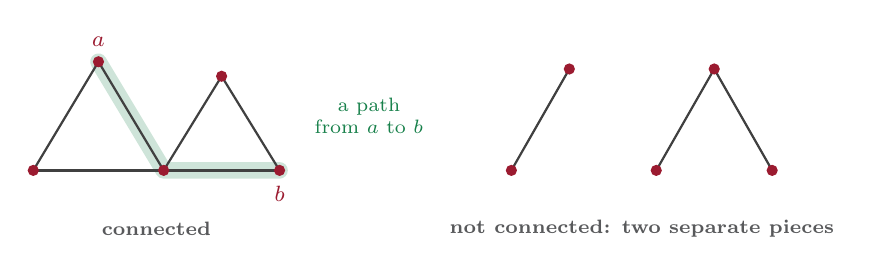
\begin{tikzpicture}[scale=0.92]
  \begin{scope}
    \coordinate (a) at (0.9,1.5); \coordinate (p) at (0,0); \coordinate (q) at (1.8,0);
    \coordinate (b) at (3.4,0);   \coordinate (r) at (2.6,1.3);
    \draw[hal] (a) -- (q) -- (b);
    \foreach \u/\v in {a/p, a/q, p/q, q/b, q/r, r/b}
      \draw[black!75, thick] (\u) -- (\v);
    \foreach \p in {a,p,q,b,r} \fill[metured] (\p) circle (2.2pt);
    \node[glab, above=2pt] at (a) {$a$}; \node[glab, below=2pt] at (b) {$b$};
    \node[capn, text=cpow, anchor=west] at (3.75,0.75) {a path\\ from $a$ to $b$};
    \node[ttl] at (1.7,-0.8) {connected};
  \end{scope}
  \begin{scope}[xshift=6.6cm]
    \coordinate (p) at (0,0); \coordinate (q) at (0.8,1.4);
    \coordinate (r) at (2.0,0); \coordinate (s) at (2.8,1.4); \coordinate (t) at (3.6,0);
    \draw[black!75, thick] (p) -- (q);
    \draw[black!75, thick] (r) -- (s) -- (t);
    \foreach \p in {p,q,r,s,t} \fill[metured] (\p) circle (2.2pt);
    \node[ttl] at (1.8,-0.8) {not connected: two separate pieces};
  \end{scope}
\end{tikzpicture}
\end{center}

\begin{ideabox}[The rows of $A$ are independent for a connected graph]
If the graph is connected, the $n-1$ rows of the reduced incidence matrix $A$ are linearly
independent: $A$ has full row rank, $\operatorname{rank} A = n - 1$.
\end{ideabox}

\textbf{Why.} Suppose some combination of the rows of $A$, with numbers $\alpha$ attached to
the nodes, gives the zero row. The reference node has no row in $A$; give it the number $\alpha = 0$. Look at
any column: a branch from node $p$ to node $q$ contributes $\alpha_p - \alpha_q$, so
$\alpha_p = \alpha_q$. Nodes joined by a branch therefore carry equal numbers. In a
connected graph every node is joined to the reference node by a path, so every $\alpha$
equals the reference value $0$. The rows are independent.

In a graph with two separate pieces the argument stops at the edge of the piece that
holds the reference node. The other piece keeps its own dependence: its rows still sum to
zero. A circuit coupled only through a transformer is like this. Joining the two pieces
with one wire makes the graph connected and changes nothing in the circuit: by KCL on a
closed surface around one piece, that wire carries no current. In EE201 all graphs are
taken to be connected.

%==============================================================
\section{KCL of a circuit graph: summary}

\begin{ideabox}[KCL in matrix form]
For a circuit whose graph is connected, with $n$ nodes and $b$ branches,
\[
  \boxed{\;A\,\Icol{\mathbf{i}} = \mathbf{0}\;}
  \qquad
  A \in \mathbb{R}^{(n-1)\times b}:\ \text{reduced incidence matrix},
  \qquad
  \Icol{\mathbf{i}} \in \mathbb{R}^{b}:\ \text{branch current vector}.
\]
These are $n-1$ \textbf{independent} KCL equations, and every other KCL equation of the
circuit follows from them.
\end{ideabox}

\begin{examplebox}[Example 7.5 --- KCL for the circuit with a 3-terminal element]
Write $A_a$, $A$ and the KCL equations for the graph of Example~7.2, with \nd3 as the
reference node.

The arrows are: branch~1 from \nd1 to \nd2, branch~2 from \nd2 to \nd3, branch~3 from \nd1
to \nd2, branch~4 from \nd3 to \nd2. Column by column:
\[
  A_a =
  \incmat{Ab}{4}{1,2,3}{%
     1 \&  0 \&  1 \&  0\\
    -1 \&  1 \& -1 \& -1\\
     0 \& -1 \&  0 \&  1\\}
  \qquad
  A =
  \begin{bmatrix}
     1 &  0 &  1 &  0\\
    -1 &  1 & -1 & -1
  \end{bmatrix} ,
\]
\[
  A\,\Icol{\mathbf{i}} = \mathbf{0}:
  \qquad
  \Icol{i_1} + \Icol{i_3} = 0, \qquad -\Icol{i_1} + \Icol{i_2} - \Icol{i_3} - \Icol{i_4} = 0 .
\]
Columns 1 and 3 are equal because branches 1 and 3 join the same nodes in the same
direction. The first equation says the current leaving \nd1 through element~1 returns
through the element's terminal at \nd1. The reference terminal of the element (at \nd2)
and the reference node of the graph (\nd3) are two separate choices.
\end{examplebox}

%==============================================================
\section*{Summary}
\addcontentsline{toc}{section}{Summary}

\begin{itemize}
  \item The $2b$ equations of a circuit split into $b$ \textbf{element equations} and $b$
        \textbf{interconnection equations} (KCL, KVL). The second group depends only on the
        wiring, that is, on the \textbf{graph}.
  \item The graph: number the branches, give each an arbitrary arrow (the current
        reference), number the nodes, and keep only dots and arrows. A $k$-terminal element
        becomes $k-1$ branches to a reference terminal.
  \item The \textbf{incidence matrix} $A_a$ ($n \times b$): $+1$ where a branch leaves a
        node, $-1$ where it enters. KCL at all nodes is $A_a\Icol{\mathbf{i}} = \mathbf{0}$.
        Each column has one $+1$ and one $-1$, so the rows sum to zero and are dependent.
  \item The \textbf{reduced incidence matrix} $A$ ($(n-1) \times b$): $A_a$ without the
        reference node's row. For a \textbf{connected} graph its rows are independent, and
        $A\Icol{\mathbf{i}} = \mathbf{0}$ gives exactly the $n-1$ independent KCL equations.
\end{itemize}

\subsection*{Next lecture}
KVL on the graph: every branch voltage is a difference of \textbf{node voltages}, which in
matrix form is $\Vcol{\mathbf{v}} = A^{T}\mathbf{e}$ --- the same matrix $A$, transposed.
Then Tellegen's theorem, which follows from $A\Icol{\mathbf{i}} = \mathbf{0}$ and
$\Vcol{\mathbf{v}} = A^{T}\mathbf{e}$ in one line.

\subsection*{Reading}
\begin{itemize}
  \item Alexander \& Sadiku, \emph{Fundamentals of Electric Circuits}, Section~2.4
        (nodes, branches and loops).
  \item Chua, Desoer \& Kuh, \emph{Linear and Nonlinear Circuits} --- circuit graphs, the
        incidence matrix and KCL in matrix form.
  \item Lecture notes and videos of Prof.\ Emre Tuna,
        \href{https://users.metu.edu.tr/etuna/ee201/}{\texttt{users.metu.edu.tr/etuna/ee201}}
        --- notes pp.~12--14; Lecture~6 video: interconnection equations $2{:}18$, circuit
        graph $4{:}00$--$7{:}55$, $k$-terminal elements $13{:}45$, KCL on the graph
        $21{:}49$, circuit matrices and the incidence matrix $26{:}04$--$30{:}40$, linear
        dependence $35{:}19$, reduced incidence matrix $40{:}45$, connected graphs
        $46{:}52$, summary $50{:}15$.
\end{itemize}

\end{document}
